\section{Introduction}
UV unwrapping is an essential step in 3D asset production, enabling textures and material details to be applied through a 2D parameterization of the mesh surface. Its quality depends critically on seam placement, i.e., where the surface is cut before flattening.  
% Manual seam placement remains tedious and expertise-demanding. Desirable seams depend not only on geometric distortion, but also on perceptual visibility, semantic part boundaries, and artist conventions. To reduce this manual effort, existing automatic UV unwrapping methods attempt to determine seams and parameterizations automatically, often through hand-crafted geometric objectives or heuristic chart construction.
Manual seam placement remains tedious and expertise-demanding. Desirable seams depend not only on geometric distortion, but also on perceptual visibility, semantic part boundaries, and artist conventions~\cite{DBLP:conf/visualization/ShefferH02,DBLP:conf/siggrapha/LucquinDB17,wang2025partuv}. To reduce this manual effort, 
%existing 
automatic UV unwrapping methods seek to generate seams and parameterizations automatically, typically by formulating UV unwrapping as a geometry-driven optimization problem.
% This motivates research on automatic UV unwrapping methods. 

% UV unwrapping is a crucial step in 3D asset production, enabling the application of textures and material details through a 2D parameterization of the mesh surface. The quality of this process hinges on seam placement—specifically, where the surface is cut before flattening. Ideal seams are influenced not only by geometric distortion but also by perceptual visibility, semantic part boundaries, and artistic conventions. As a result, automatic UV unwrapping methods have been developed to replace manual seam placement, alleviating the time-consuming and expertise-intensive nature of the task.
 
Most existing approaches are based on per-object optimization with geometric distortion objectives, such as angle or area preservation~\cite{levy2002least, sheffer2005abf, rabinovich2017scalable, li2018optcuts}, while more recent methods, such as PartUV~\cite{wang2025partuv}, additionally incorporate semantic part segmentation as a proxy for structured chart layouts. However, handcrafted objectives and semantic proxies are not always well aligned with the industrial production requirements. 
As a result, layouts produced by current methods often fail to place seams in ways that support practical texture authoring, such as avoiding visually salient regions and preserving texture continuity across important surface areas.
% deviate substantially from those created by professional artists and remain unsuitable for production use. 
%
% In particular, they often fail to place seams in ways that support practical texture authoring.
% , such as avoiding visually salient regions and preserving texture continuity across important surface areas.
For the example of a dog model (see Fig. \ref{fig:artist}), artists typically avoid placing seams on the face. In contrast, methods such as xatlas~\cite{young2019xatlas} and PartUV~\cite{wang2025partuv} often introduce excessive seams in this region to reduce distortion, which disrupts texture continuity and increases the risk of visible artifacts.
%
This can be attributed to the gap between explicit optimization objectives and the complex seam design preferences encountered in real-world settings, where the latter often involve practical, perceptual, semantic, and geometric factors shaped by visual experience and production requirements.
Consequently, per-object optimization is inherently constrained. These observations motivate a data-driven formulation that learns seam placement directly from artist-authored examples. 


\begin{figure}
    \centering
    \vspace{-6mm}
    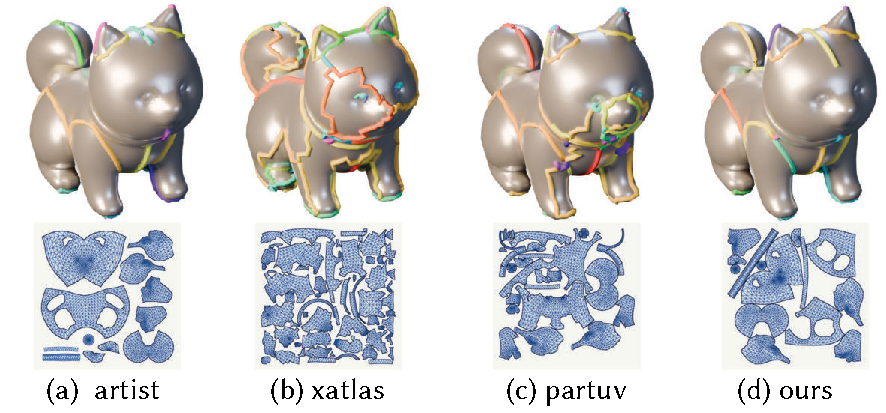
\includegraphics[width=\linewidth]{figures/artist.pdf}
    \caption{
    \textbf{Comparison with artist-authored seam placement.}
    (a) Artist-authored seams avoid salient regions (e.g., the face), favoring inconspicuous boundaries.
    (b-c) Distortion-oriented methods such as xatlas and PartUV produce seam layouts that differ substantially from the artist-authored reference, with seams often appearing in visually important facial regions.
    (d) \methodname{} better matches the artist-authored seam distribution, preserving the face while placing cuts along more natural boundaries.
    }
    \vspace{-6mm}
    \label{fig:artist}
\end{figure}


 

% To this end, we propose \textit{\methodname{}}, which formulates UV seam generation as a distribution-fitting problem on the mesh graph. 
To this end, we propose \textit{\methodname{}}, which formulates surface seam cutting as a conditional generation problem on the mesh graph, learning the distribution of artist-authored seam layouts conditioned on the input geometry.
Seam generation is challenging because seam edges occupy only a small fraction of all mesh edges, yet should still respect geometry, semantics, artist conventions, and topology on irregular mesh connectivity.  
% Instead of independently identifying seams from all edges, we adopt flow matching~\cite{lipman2023flow} as our generative formulation, learning to transform random edge-wise noise into a structured seam probability field. 
Instead of independently identifying seams from all edges, we adopt flow matching~\cite{lipman2023flow} as our generative formulation, learning to transform random edge-wise noise into a coherent binary seam indicator on the mesh graph.
A key challenge is that typical Transformer architectures are designed for sequential modeling and are therefore better suited to representations such as point clouds, without naturally accounting for mesh topology. However, seam decisions depend on both global context, which coordinates cuts into coherent layouts across the entire shape, and local geometric cues, such as dihedral angles and curvature, which determine where seams should be placed in a topology-aware manner.
%
To enable mesh-native learning, we design a Mesh Transformer backbone that interleaves local graph attention over mesh edges with global self-attention across vertices, capturing both fine-grained geometric cues and long-range topological coherence.
% 
% To support localized control, we further exploit the training-free inpainting capability of flow models for conditional seam editing. 
% Given sparse user constraints, such as seam-free regions or prescribed cut edges, we clamp the specified edges during sampling and re-generate the remaining seam layout using the same learned flow model. 
% This allows \methodname{} to complete user-guided layouts while preserving artist-like seam statistics. 
% Beyond manual editing, we instantiate this conditional generation principle as a validity-aware self-refinement procedure. 
% When an initial layout induces an invalid UV atlas, \methodname{} anchors the reliable seams and selectively re-samples the problematic subgraph under these constraints. 
% This inference-time correction improves atlas validity while preserving the global seam organization and artist-authored statistics learned by the model.
To support localized control, we further exploit the learned flow model as a training-free conditional prior. 
Given sparse user constraints, such as seam-free regions or prescribed cut edges, \methodname{} clamps the specified edges during sampling and regenerates the remaining seam layout. 
The same mechanism also enables overlap self-refinement: when an initial layout produces invalid UV overlaps, we fix the reliable seams and resample only the problematic local region. 
This enables constrained editing and inference-time correction without additional training or a separate repair model.
Together, these designs enable \methodname{} to generate seam layouts that better match \textit{artist-authored priors} while remaining robust in practical UV unwrapping scenarios.

In summary, our contributions are as follows:
\begin{itemize}
    % \item We formulate UV seam cutting as mesh-edge seam generation rather than distortion-driven optimization, and propose \methodname{}, the first flow-matching-based framework for learning artist-authored seam layout priors from real-world UV data.
    \item We formulate UV seam cutting as mesh-edge seam generation and propose \methodname{}, the first flow-matching framework that learns artist-authored seam layout priors from real-world UV data.
    \item We develop a mesh-native Mesh Transformer for seam prediction on mesh graphs, and reuse the learned flow model as a training-free conditional prior for constraint-guided completion and overlap self-refinement.
    \item We demonstrate that by learning priors from professional seam  data, \methodname{} produces better artist-aligned UV layouts with superior perceptual quality than baselines.
\end{itemize}
